\nextslide{1. Basic principles}
\begin{enumerate}
\item Some basics
\item Jack
\item Interacting with the user
\item Interacting with the prover
\end{enumerate}

\nextslide{Some basics}
\small
The {\purple Java Modelling Language} (JML)
is used to annotate the Java programs we want to verify with 
Jack or ESC/Java.\\
Jack and ESC/Java use a {\purple weakest precondition calculus} to generate
the proof obligations.\\
In JML you can express loop invariants, assertions method's
pre and post conditions.\\
JML has a really large syntax so every tool (except maybe JMLrac)
implements only a {\purple portion} of its syntax.


\nextslide{Jack}
\small
\blist
\item At first single prover (B)
\item Multi-prover interface (Simplify, Coq, PVS)
\item Fully integrated in {\purple Eclipse} as a plugin, and use a 
{\purple plugin architecture} to include new provers
\elist
\begin{center}
\includegraphics[width= \linewidth]{jack.ps}
\end{center}

\nextslide{Some features}\small
Jack supports most JML functionnalities although the parser is old.\\
It adds 2 construct:
\blist
\item {\tt loop\_modify} keyword
\item {\tt native} keyword for JML annotations\\
\elist

Jack's IDE is also used by Mariela Pavlova's 
weakest precondition calculus over bytecode
